%%%%%%%%%%%%%%%%%%%%%%%%%%%%%%%%%%%%%%%%%
% Classicthesis Typographic Thesis
% LaTeX Template
% Version 1.1 (4/8/12)
%!TEX encoding = UTF-8 Unicode
% This template has been downloaded from
% http://www.LaTeXTemplates.com
%
% Original author:
% André Miede (http://www.miede.de)
%
% License:
% CC BY-NC-SA 3.0 (http://creativecommons.org/licenses/by-nc-sa/3.0/)
%
% General Tips:
% 1) Make sure to edit the classicthesis-config.file
% 2) New enumeration (A., B., C., etc in small caps): \begin{aenumerate} \end{aenumerate}
% 3) For margin notes: \marginpar or \graffito{}
% 4) Do not use bold fonts in this style, it is designed around them
% 5) Use tables as in the examples
% 6) See classicthesis-preamble.sty for useful commands
%    
%%%%%%%%%%%%%%%%%%%%%%%%%%%%%%%%%%%%%%%%%

%----------------------------------------------------------------------------------------
%	PACKAGES AND OTHER DOCUMENT CONFIGURATIONS
%----------------------------------------------------------------------------------------


\documentclass[
		oneside,openright,titlepage,numbers=noenddot,headinclude,%1headlines,
                footinclude=true,cleardoublepage=empty,
                BCOR=0mm,paper=a4,fontsize=11pt, % Binding correction, paper type and font size
                ngerman,american, % Languages
                ]{scrreprt} 
                
               
\hyphenpenalty=1000
                

% Includes the file which contains all the document configurations and packages - make sure to edit this file
%%%%%%%%%%%%%%%%%%%%%%%%%%%%%%%%%%%%%%%%%
% Thesis Configuration File
%
% The main lines to change in this file are in the DOCUMENT VARIABLES
% section, the rest of the file is for advanced configuration.
%
%%%%%%%%%%%%%%%%%%%%%%%%%%%%%%%%%%%%%%%%%

%----------------------------------------------------------------------------------------
%	DOCUMENT VARIABLES
%	Fill in the lines below to enter your information into the thesis template
%	Each of the commands can be cited anywhere in the thesis
%----------------------------------------------------------------------------------------

% Remove drafting to get rid of the '[ Date - classicthesis version 4.0 ]' text at the bottom of every page
\PassOptionsToPackage{eulerchapternumbers,listings, pdfspacing, subfig,beramono,eulermath,parts}{classicthesis}
% Available options: drafting parts nochapters linedheaders eulerchapternumbers beramono eulermath pdfspacing minionprospacing tocaligned dottedtoc manychapters listings floatperchapter subfig
% Adding 'dottedtoc' will make page numbers in the table of contents flushed right with dots leading to them

\newcommand{\myTitle}{Enhancing Content Discovery: an Evaluation and Classification Perspective\xspace}
\newcommand{\myDegree}{This thesis submitted to University College Dublin in fulfilment of the requirements for the degree of Research Masters\xspace}
\newcommand{\myName}{Humberto Jes�s Corona Pamp�n\xspace}
\newcommand{\myID}{UCD student number: 2222222 \xspace}
\newcommand{\mySupervisor}{Supervisor: Dr. Michael P. O'Mahony\xspace}
\newcommand{\myHOS}{Head of School: Prof. P�draig Cunningham\xspace}
\newcommand{\myFaculty}{School of Computer Science and Informatics\xspace}
\newcommand{\myDepartment}{\xspace}
\newcommand{\myUni}{University College Dublin\xspace}
\newcommand{\myLocation}{Dublin\xspace}
\newcommand{\myTime}{September 2014\xspace}
\newcommand{\myVersion}{version 1.0.0 \xspace}

%----------------------------------------------------------------------------------------
%	USEFUL COMMANDS
%----------------------------------------------------------------------------------------

\newcommand{\ie}{i.\,e.}
\newcommand{\Ie}{I.\,e.}
\newcommand{\eg}{e.\,g.}
\newcommand{\Eg}{E.\,g.} 

\newcounter{dummy} % Necessary for correct hyperlinks (to index, bib, etc.)
\providecommand{\mLyX}{L\kern-.1667em\lower.25em\hbox{Y}\kern-.125emX\@}

%----------------------------------------------------------------------------------------
%	PACKAGES
%----------------------------------------------------------------------------------------

\usepackage{lipsum} % Used for inserting dummy 'Lorem ipsum' text into the template

%------------------------------------------------
 
\PassOptionsToPackage{latin9}{inputenc} % latin9 (ISO-8859-9) = latin1+"Euro sign"
\usepackage{inputenc}
 
 %------------------------------------------------

%\PassOptionsToPackage{ngerman,american}{babel}  % Change this to your language(s)
% Spanish languages need extra options in order to work with this template
%\PassOptionsToPackage{spanish,es-lcroman}{babel}
\usepackage{babel}

%------------------------------------------------			

\PassOptionsToPackage{square,numbers}{natbib}
 \usepackage{natbib}
 
 %------------------------------------------------

\PassOptionsToPackage{fleqn}{amsmath} % Math environments and more by the AMS 
 \usepackage{amsmath}
 
 %------------------------------------------------

\PassOptionsToPackage{T1}{fontenc} % T2A for cyrillics
\usepackage{fontenc}

%------------------------------------------------

\usepackage{xspace} % To get the spacing after macros right

%------------------------------------------------

\usepackage{mparhack} % To get marginpar right

%------------------------------------------------

\usepackage{fixltx2e} % Fixes some LaTeX stuff 

%------------------------------------------------

\PassOptionsToPackage{smaller}{acronym} % Include printonlyused in the first bracket to only show acronyms used in the text
\usepackage{acronym} % nice macros for handling all acronyms in the thesis

%------------------------------------------------

%\renewcommand*{\acsfont}[1]{\textssc{#1}} % For MinionPro
\renewcommand{\bflabel}[1]{{#1}\hfill} % Fix the list of acronyms

%------------------------------------------------

\PassOptionsToPackage{pdftex}{graphicx}
\usepackage{graphicx} 

%----------------------------------------------------------------------------------------
%	FLOATS: TABLES, FIGURES AND CAPTIONS SETUP
%----------------------------------------------------------------------------------------

\usepackage{tabularx} % Better tables
\setlength{\extrarowheight}{3pt} % Increase table row height
\newcommand{\tableheadline}[1]{\multicolumn{1}{c}{\spacedlowsmallcaps{#1}}}
\newcommand{\myfloatalign}{\centering} % To be used with each float for alignment
\usepackage{caption}
\captionsetup{format=hang,font=small}
\usepackage{subfig}  

%----------------------------------------------------------------------------------------
%	CODE LISTINGS SETUP
%----------------------------------------------------------------------------------------

\usepackage{listings} 
%\lstset{emph={trueIndex,root},emphstyle=\color{BlueViolet}}%\underbar} % for special keywords
\lstset{language=[LaTeX]Tex, % Specify the language for listings here
keywordstyle=\color{RoyalBlue}, % Add \bfseries for bold
basicstyle=\small\ttfamily, % Makes listings a smaller font size and a different font
%identifierstyle=\color{NavyBlue}, % Color of text inside brackets
commentstyle=\color{Green}\ttfamily, % Color of comments
stringstyle=\rmfamily, % Font type to use for strings
numbers=left, % Change left to none to remove line numbers
numberstyle=\scriptsize, % Font size of the line numbers
stepnumber=5, % Increment of line numbers
numbersep=8pt, % Distance of line numbers from code listing
showstringspaces=false, % Sets whether spaces in strings should appear underlined
breaklines=true, % Force the code to stay in the confines of the listing box
%frameround=ftff, % Uncomment for rounded frame
frame=single, % Frame border - none/leftline/topline/bottomline/lines/single/shadowbox/L
belowcaptionskip=.75\baselineskip % Space after the "Listing #: Desciption" text and the listing box
}

%----------------------------------------------------------------------------------------
%	HYPERREFERENCES
%----------------------------------------------------------------------------------------

\PassOptionsToPackage{pdftex,hyperfootnotes=false,pdfpagelabels}{hyperref}
\usepackage{hyperref}  % backref linktocpage pagebackref
\pdfcompresslevel=9
\pdfadjustspacing=1

\hypersetup{
% Uncomment the line below to remove all links (to references, figures, tables, etc)
%draft, 
colorlinks=true, linktocpage=true, pdfstartpage=3, pdfstartview=FitV,
% Uncomment the line below if you want to have black links (e.g. for printing black and white)
%colorlinks=false, linktocpage=false, pdfborder={0 0 0}, pdfstartpage=3, pdfstartview=FitV, 
breaklinks=true, pdfpagemode=UseNone, pageanchor=true, pdfpagemode=UseOutlines,
plainpages=false, bookmarksnumbered, bookmarksopen=true, bookmarksopenlevel=1,
hypertexnames=true, pdfhighlight=/O, urlcolor=webbrown, linkcolor=RoyalBlue, citecolor=webgreen,
%------------------------------------------------
% PDF file meta-information
pdftitle={\myTitle},
pdfauthor={\textcopyright\ \myName, \myUni, \myFaculty},
pdfsubject={},
pdfkeywords={},
pdfcreator={pdfLaTeX},
pdfproducer={LaTeX with hyperref and classicthesis}
%------------------------------------------------
}   

%----------------------------------------------------------------------------------------
%	BACKREFERENCES
%----------------------------------------------------------------------------------------

\usepackage{ifthen} % Allows the user of the \ifthenelse command
\newboolean{enable-backrefs} % Variable to enable backrefs in the bibliography
\setboolean{enable-backrefs}{false} % Variable value: true or false

\newcommand{\backrefnotcitedstring}{\relax} % (Not cited.)
\newcommand{\backrefcitedsinglestring}[1]{(Cited on page~#1.)}
\newcommand{\backrefcitedmultistring}[1]{(Cited on pages~#1.)}
\ifthenelse{\boolean{enable-backrefs}} % If backrefs were enabled
{
\PassOptionsToPackage{hyperpageref}{backref}
\usepackage{backref} % to be loaded after hyperref package 
\renewcommand{\backreftwosep}{ and~} % separate 2 pages
\renewcommand{\backreflastsep}{, and~} % separate last of longer list
\renewcommand*{\backref}[1]{}  % disable standard
\renewcommand*{\backrefalt}[4]{% detailed backref
\ifcase #1 
\backrefnotcitedstring
\or
\backrefcitedsinglestring{#2}
\else
\backrefcitedmultistring{#2}
\fi}
}{\relax} 

%----------------------------------------------------------------------------------------
%	AUTOREFERENCES SETUP
%	Redefines how references in text are prefaced for different 
%	languages (e.g. "Section 1.2" or "section 1.2")
%----------------------------------------------------------------------------------------

\makeatletter
\@ifpackageloaded{babel}
{
\addto\extrasamerican{
\renewcommand*{\figureautorefname}{Figure}
\renewcommand*{\tableautorefname}{Table}
\renewcommand*{\partautorefname}{Part}
\renewcommand*{\chapterautorefname}{Chapter}
\renewcommand*{\sectionautorefname}{Section}
\renewcommand*{\subsectionautorefname}{Section}
\renewcommand*{\subsubsectionautorefname}{Section}
}
\addto\extrasngerman{
\renewcommand*{\paragraphautorefname}{Absatz}
\renewcommand*{\subparagraphautorefname}{Unterabsatz}
\renewcommand*{\footnoteautorefname}{Fu\"snote}
\renewcommand*{\FancyVerbLineautorefname}{Zeile}
\renewcommand*{\theoremautorefname}{Theorem}
\renewcommand*{\appendixautorefname}{Anhang}
\renewcommand*{\equationautorefname}{Gleichung}
\renewcommand*{\itemautorefname}{Punkt}
}
\providecommand{\subfigureautorefname}{\figureautorefname} % Fix to getting autorefs for subfigures right
}{\relax}
\makeatother

%----------------------------------------------------------------------------------------

\usepackage{classicthesis} 

%----------------------------------------------------------------------------------------
%	CHANGING TEXT AREA 
%----------------------------------------------------------------------------------------

%\linespread{1.05} % a bit more for Palatino
%\areaset[current]{312pt}{761pt} % 686 (factor 2.2) + 33 head + 42 head \the\footskip
%\setlength{\marginparwidth}{7em}%
%\setlength{\marginparsep}{2em}%

%----------------------------------------------------------------------------------------
%	USING DIFFERENT FONTS
%----------------------------------------------------------------------------------------

%\usepackage[oldstylenums]{kpfonts} % oldstyle notextcomp
%\usepackage[osf]{libertine}
%\usepackage{hfoldsty} % Computer Modern with osf
%\usepackage[light,condensed,math]{iwona}
%\renewcommand{\sfdefault}{iwona}
%\usepackage{lmodern} % <-- no osf support :-(
%\usepackage[urw-garamond]{mathdesign} <-- no osf support :-(

\usepackage{multirow}
\usepackage{algorithm}
\usepackage{algorithmic}
\usepackage{parskip}
\usepackage{blindtext}

 
 \begin{document}
\frenchspacing % Reduces space after periods to make text more compact
\raggedbottom % Makes all pages the height of the text on that page
\selectlanguage{american} % Select your default language - e.g. american or ngerman
\pagenumbering{roman} % Roman page numbering prior to the start of the thesis content (i, ii, iii, etc)
\pagestyle{plain} % Suppress headers for the pre-content pages
%\renewcommand*{\bibname}{new name} % Uncomment to change the name of the bibliography
%\setbibpreamble{} % Uncomment to include a preamble to the bibliography - some text before the reference list starts

%----------------------------------------------------------------------------------------
%	PRE-CONTENT THESIS PAGES
%----------------------------------------------------------------------------------------


% Title Page

\begin{titlepage}

\begin{addmargin}[-1cm]{-3cm}
\begin{center}
\large

\hfill
\vfill

\begingroup
\color{Maroon}\spacedallcaps{\myTitle} \\ \bigskip % Thesis title
\endgroup

\spacedlowsmallcaps{\myName} \\% Your name
\myID
\vfill

\vspace{4cm}


\includegraphics[width=3cm]{gfx/logo} \\ \medskip % Picture

\myDegree \\ \bigskip
\myFaculty \\ 
\myUni \\  \bigskip


\myHOS \\  
\bigskip
\mySupervisor \\ 

\vspace{6cm}

\myTime\ % Time and version

\vfill

\end{center}
\end{addmargin}

\end{titlepage} % Main title page 
\cleardoublepage
% Back of the title page

\thispagestyle{empty}

\hfill

\vfill

\noindent\myName: \\ \textit{\myTitle,} %\myDegree, 
\textcopyright\ \myTime

% You may wish to do something with the back of the title page, such as including your supervisors, location or time frame of the work. Below is an example of doing so although you may want to tweak it to your liking.

%\bigskip

%\noindent\spacedlowsmallcaps{Supervisors}: \\
%\myProf \\
%\myOtherProf \\ 
%\mySupervisor

%\medskip \\

%\noindent\spacedlowsmallcaps{Location}: \\
%\myLocation

%\medskip \\

%\noindent\spacedlowsmallcaps{Time Frame}: \\
%\myTime
 % Back of the title page
\cleardoublepage
%*******************************************************
% Dedication
%*******************************************************
\thispagestyle{empty}
%\phantomsection 
\refstepcounter{dummy}
\pdfbookmark[1]{Dedication}{Dedication}

\vspace*{\fill}

\begin{center}
    Without music,   life would be a mistake. \\ \medskip
    --- Friedrich Nietzsche.   
\end{center}

\vspace{5cm}

\begin{center}
   \blindtext
\end{center}

\vspace*{\fill} % Dedication page
\cleardoublepage
% Abstract

\pdfbookmark[1]{Abstract}{Abstract} % Bookmark name visible in a PDF viewer

\begingroup
\let\clearpage\relax
\let\cleardoublepage\relax
\let\cleardoublepage\relax

\chapter*{Abstract} % Abstract nam

\blindtext

\blindtext

\blindtext

\endgroup			
 % Abstract page
\cleardoublepage
% Declaration

\refstepcounter{dummy}
\pdfbookmark[0]{Declaration}{declaration} % Bookmark name visible in a PDF viewer

\chapter*{Declaration} % Declaration section text

\thispagestyle{empty}

I herby certify that the submitted work is my own work, was completed while registered as a candidate for the degree stated on the Title Page, and I have not obtained a degree elsewhere on the basis of the research presented in this submitted work.
\bigskip
 
%\noindent\textit{\myLocation, \myTime}

\bigskip

\begin{flushright}
\begin{tabular}{m{8cm}}
\\ \hline
\centering\myName, \\ \today \\
\end{tabular}
\end{flushright}
 % Publications from the thesis page
\cleardoublepage
% Publications - a page listing research articles written using content in the thesis

\pdfbookmark[1]{Publications}{Publications} % Bookmark name visible in a PDF viewer

\chapter*{Publications} % Publications page text

Some ideas and figures have appeared previously in the following thesis publications:

\bigskip

Humberto Jes\'{u}s Corona Pamp\'{i}n , Houssem Jerbi, and Michael P. O'Mahony. ``Evaluating the Relative Performance of Neighbourhood-Based Recommender Systems.'' In Proceedings of the 3rd Spanish Conference on Information Retrieval, pages 25-36, 2014.

Humberto Jes\'{u}s Corona Pamp\'{i}n and Michael P. O'Mahony. ``A Mood-based Genre Classification of Television Content''. In proceedings of the first ACM Workshop on Recommendation Systems for Television and Online Video (to be published in October 2014).

\bigskip

 % Publications from the thesis page
\cleardoublepage
% Acknowledgements


\vspace*{\fill}
{\Large This work is supported by Science Foundation Ireland through the CLARITY Centre for Sensor Web Technologies  under grant number XXXXXXXXX.}

\begin{figure}[h!]
  \centering
    
\includegraphics[width=1\textwidth]{figures/ack}
    \end{figure}
\vspace*{\fill}



\newpage 

\pdfbookmark[1]{Acknowledgements}{Acknowledgements} % Bookmark name visible in a PDF viewer

%----------------------------------------------------------------------------------------

\begingroup


\chapter*{Acknowledgements} % Acknowledgements section text

\blindtext

\blindtext



\endgroup % Acknowledgements page
\cleardoublepage
%\pagestyle{scrheadings} % Show chapter titles as headings
% DELETED THE HEADINGS BECAUSE IT WAS GIVING ME PROBLEMS WITH THE LONG HEADINGS!
\cleardoublepage% Table of Contents - List of Tables/Figures/Listings and Acronyms

\refstepcounter{dummy}

\pdfbookmark[1]{\contentsname}{tableofcontents} % Bookmark name visible in a PDF viewer

\setcounter{tocdepth}{2} % Depth of sections to include in the table of contents - currently up to subsections

\setcounter{secnumdepth}{3} % Depth of sections to number in the text itself - currently up to subsubsections

\manualmark
\markboth{\spacedlowsmallcaps{\contentsname}}{\spacedlowsmallcaps{\contentsname}}
\tableofcontents 
\automark[section]{chapter}
\renewcommand{\chaptermark}[1]{\markboth{\spacedlowsmallcaps{#1}}{\spacedlowsmallcaps{#1}}}
\renewcommand{\sectionmark}[1]{\markright{\thesection\enspace\spacedlowsmallcaps{#1}}}

\clearpage

\begingroup 
\let\clearpage\relax
\let\cleardoublepage\relax
\let\cleardoublepage\relax

%----------------------------------------------------------------------------------------
%	List of Figures
%----------------------------------------------------------------------------------------

\refstepcounter{dummy}
%\addcontentsline{toc}{chapter}{\listfigurename} % Uncomment if you would like the list of figures to appear in the table of contents
\pdfbookmark[1]{\listfigurename}{lof} % Bookmark name visible in a PDF viewer

\listoffigures

\vspace*{8ex}
\newpage

%----------------------------------------------------------------------------------------
%	List of Tables
%----------------------------------------------------------------------------------------

\refstepcounter{dummy}
%\addcontentsline{toc}{chapter}{\listtablename} % Uncomment if you would like the list of tables to appear in the table of contents
\pdfbookmark[1]{\listtablename}{lot} % Bookmark name visible in a PDF viewer

\listoftables
        
\vspace*{8ex}
\newpage
    
%%----------------------------------------------------------------------------------------
%%	List of Listings
%%---------------------------------------------------------------------------------------- 
%
%\refstepcounter{dummy}
%%\addcontentsline{toc}{chapter}{\lstlistlistingname} % Uncomment if you would like the list of listings to appear in the table of contents
%\pdfbookmark[1]{\lstlistlistingname}{lol} % Bookmark name visible in a PDF viewer
%
%\lstlistoflistings 
%
%\vspace*{8ex}
%\newpage
       
%----------------------------------------------------------------------------------------
%	Acronyms
%----------------------------------------------------------------------------------------

\refstepcounter{dummy}



                   
\endgroup

\cleardoublepage % Contents, list of figures/tables/listings and acronyms
\pagenumbering{arabic} % Arabic page numbering for thesis content (1, 2, 3, etc)
\cleardoublepage % Avoids problems with pdfbookmark

%----------------------------------------------------------------------------------------
%	THESIS CONTENT - CHAPTERS
%----------------------------------------------------------------------------------------

% Chapter 1

\chapter{Introduction}\label{ch:introduction} % For referencing the chapter elsewhere, use \autoref{ch:introduction} 


The Internet can be defined as  \emph{a global system of interconnected computer networks}, and  since the appearance of the World Wide Web (WWW) in 1989, it has been constantly changing and growing, becoming a vital part of our lives in  contemporary society \cite{Morris1996}.  Before the ubiquitous presence of the Internet and the WWW,  people had access to books only in libraries, films in cinemas or rental shops, and records were sold in physical format. Thus,  access was limited and difficult. As physical storage was needed, it was impossible to find every book (film or record) in the same physical space at once. Nowadays the access problem is solved, and people have access to these and many other products and services through smart devices connected to the Internet. However, the solution of the information access problem led to an information overload problem. For example, in the 80's a common user had access to hundreds of songs, while nowadays streaming services like Spotify\footnote{\url{http://www.spotify.com}} provide access to dozens of millions of songs.  Moreover, traditional ways of content discovery such as the so-called \emph{word of mouth} on physical social networks (neighbours, family or friends) have been translated into their online counterparts (Facebook\footnote{\url{http://facebook.com}}, Twitter\footnote{\url{http://twitter.com}}, etc.), changing the way content is discovered and consumed. 

As access to media becomes easier, and the amount of user generated content builds up, there is an increasing difficulty when dealing with the vast amount of information which is available. Finding a new movie to watch, discovering new bands to listen to, or deciding whom to follow in an online social network is becoming increasingly difficult for the user. In fact, we often find ourselves overloaded with information and choice. Therefore, there is a need for a new class of  intelligent systems that help us to navigate through all this information, by automatically identifying  relevant content and filtering  that which is irrelevant. Recommender systems \cite{Aman2010, Ricci2011, Levy2010a, Resnick1997, Schafer1999} perform this task by learning the products and services we like, the news articles we find interesting, or the music we listen to. All this knowledge is then applied to personalise the user experience in different services; from advertising to clothes recommender systems, from movie recommender systems to music discovery. Thus, much of the content that users access on the internet can be filtered according to their needs in a personalised fashion. 


Recommender systems are a class of information filtering systems which aim to present information in a personalised fashion, aiding the user to browse large collection of items, i.e., scientific articles \cite{Toscher2009} or movies  \cite{Wang2011, Golbeck2006} . These type of  systems have been widely exploited in the last decade, and are often found on internet sites dealing with large amounts of information such as Netflix\footnote{\url{http://www.netflix.com}} (video streaming platform) or Spotify (music streaming platform). Moreover, the concept of recommender system is very broad. For example, they have been used in collaborative search using reputation systems \cite{Mahony2010},  to get recommendations of people to follow in social networks \cite{Hannon2010}, to classify news feeds \cite{Phelan2012, Esparza2013} or to help users navigate through large collections of products reviews in an e-commerce scenario \cite{Dong2012}, among many other applications.


Figure \ref{fig:netflix1} shows the Netflix web interface,  which is completely personalised. For example, the movies in the \emph{top picks} row are shown based on the user's past behaviour, while the second row shows similar items to a previously watched (and liked) television show.


\begin{figure}[h!] 
  \centering
    
\includegraphics[width=1\textwidth]{figures/netflix.png}
  \caption{The Netflix user interface shows different recommendations streams.}
   \label{fig:netflix1}
\end{figure}

Figure \ref{fig:amazon1} shows the non-personalised recommendations generated by the popular e-commerce site Amazon\footnote{ \url{http://www.amazon.com}}, based on the "people who bought this also bought that" model of recommendation, not taking in account the user's previous interaction with the system.


\begin{figure}[h!] 
  \centering
    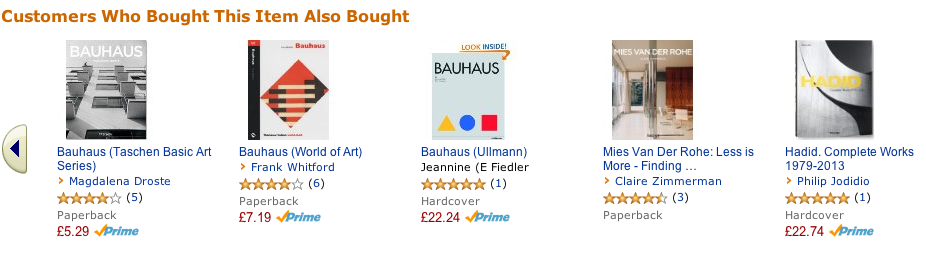
\includegraphics[width=1\textwidth]{figures/amazon1}
  \caption{Amazon present users with non-personalised recommendations of similar items calculated by shopping co-ocurrence.}
   \label{fig:amazon1}
\end{figure}


Recommender systems can be classified according to the information they use when generating recommendations. \emph{Collaborative recommender systems (CF)} \cite{Sarwara, Koren2008, Bell2007} use the wisdom of the crowd to identify trends on how users interact with the system. They are able to find like-minded users and use that information to make recommendations, relying only on preference data from the users in the system. These type of algorithms are widely present in commercial systems such as the e-commerce platform Amazon \cite{Linden2003}, which uses item-to-item collaborative recommendations. Moreover, they have proven to be accurate, specially thanks to advances developed in the context of the Netflix Prize \cite{Bennett2007}. \emph{Content-based Filtering (CBF) recommender systems} \cite{Meteren, Lops2011,  Pazzani2007}  utilise user feedback provided by users to generate recommendations of similar items to those users have liked in the past, by analysing the content metadata. These type of systems are particularly useful in cases where the access to other user's preferences is limited but rich metadata is available, for example in the case of television recommendations \cite{Blanco-Fernandez2008}. \emph{Hybrid systems} \cite{Modeling2002, Bostandjiev2012} usually combine content-based with collaborative filtering approaches, with the aim of obtaining a better performance than with a single approach, while reducing the drawbacks of each approach. The most commonly used hybrid approaches are \emph{weighted hybrid recommenders}, \emph{switching hybrid recommenders} and \emph{mixed hybrid recommenders}, as described in \cite{Modeling2002}.

An interesting and widely studied area of recommender systems is evaluation \cite{Herlocker2004, Shani}. Traditionally, recommender systems evaluation focused on measuring accuracy. However, in recent times the focus has extended to measure recommender systems properties  beyond accuracy \cite{Konstan2012, McNee2006a} such as diversity, popularity, novelty or serendipity. Performing an evaluation that considers all these facets is necessary to better understand all the factors that affect the performance of this type of systems and how they affect the enhancement of content discovery. Moreover, there is a growing interest in studying the evaluation of recommender systems considering not only \emph{offline evaluation} experiment, but also \emph{user studies} and \emph{A/B testing} \cite{Shani}.


The music industry has dramatically changed in the last decades and has become an example of a scenario where information overload is a critical problem. The formats and devices in which music is played have changed several times;  from vinyl, to cassettes, CDs, mp3 players and finally to smartphones. Products like the iPod\footnote{\url{https://www.apple.com/ipod/}} (first released in 2001) or services like Napster\footnote{\url{http://ie.napster.com/start}} (a P2P music sharing service first released in 2000) challenged the traditional music distribution channels such as record stores and radios. More recently, services like Last.FM\footnote{\url{http://www.last.fm/}} (which allows users to track and tag all the music listened to), Spotify or  rdio\footnote{\url{http://www.rdio.com/}}  are disrupting the traditional music business model, based in the purchase of albums in physical stores, shifting users towards a monthly payment model with unlimited access to vast music catalogs. In this context, music discovery, classification and recommendation has become a more important part of each of these products, driving  research both in industry and academia \cite{Levy2010a, Celma2011, Aman2010, Celma2009}. 

 \begin{figure}[h!]
\centering
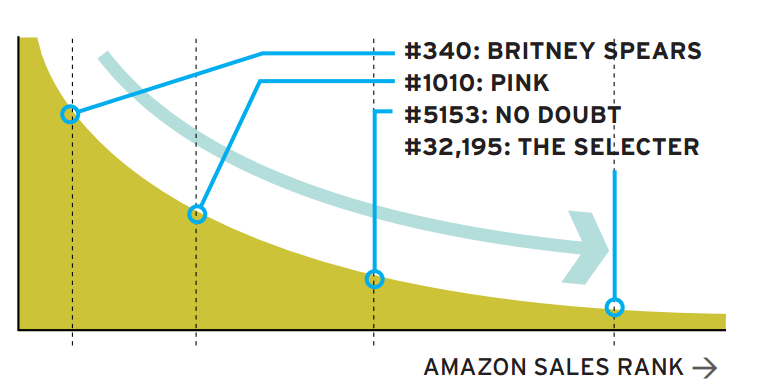
\includegraphics[width=1 \textwidth]{figures/top_amazon}
\caption{Sales per artist on the e-commerce website Amazon.com, from the 2010 Wired Magazine article \emph{The Long Tail}, by Chris Anderson \cite{Anderson2004}.}
\label{fig:top_mine}
\end{figure}


Even when effort has been put into enabling music discovery, overall listening behaviour has, however, not changed, and still follows a long tail distribution. Thus, a very reduced amount of artists are extremely popular, while there is a  long list of artists and songs that rarely get sold or listened to. An example is pictured in Figure \ref{fig:top_mine}, which shows total sales per artist on the e-commerce site Amazon (vertical axis) sorted by popularity (horizontal axis). Here, the total number of records sold by artists like \emph{Britney Spears} are several orders of magnitude bigger than other less popular artists such as \emph{The Selecter}. Thus, the long tail of artists needs to be exploited when generating recommendations to increase sales, artist visibility, and provide novel recommendations to the consumer.

 
The problem of music discovery has been widely studied in recent times and several reviews of the field have been published \cite{Song2012, Celma2009, Celma2011}.  One of the approaches to solve the information overload in this field is by automatically classifying music, which allows sorting large music collections or automatically generating playlist and recommendations. This type of approach has been successfully used to generate music recommendations based on mood  \cite{Han2009} and genre \cite{Hu2012}. For example, Figure \ref{fig:spotify_recs} shows the Spotify desktop application interface, where playlists are classified according to their moods and genres.

%The classification problem is often divided according to the type of data available in the training process. In \emph{supervised learning} \cite{Mccallum1997, IanH.Witten2005} the classifier uses labeled data to learn a model, and then classifies new instances based on that model. In  \emph{unsupervised learning}  \cite{Cord2001, Barlow1989} (often referred as clustering)  the data is partitioned without using predefined class labels, thus it is the algorithm which decides how to best partition the data into a predefined number of clusters.  


  \begin{figure}[h!]
\centering
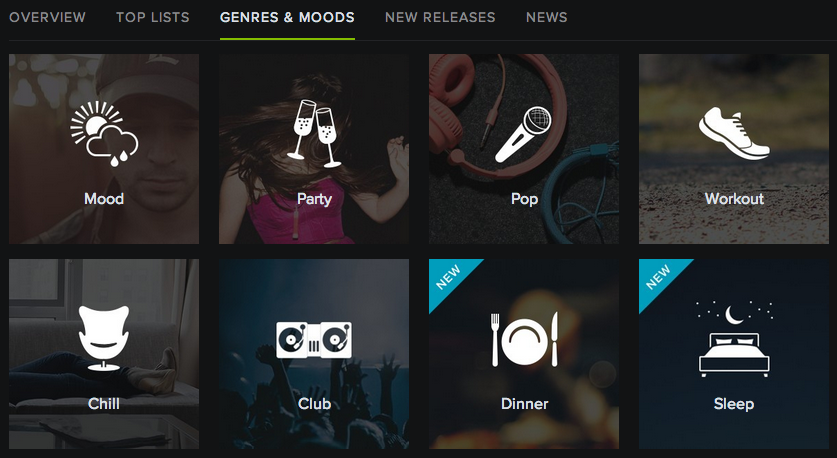
\includegraphics[width=1 \textwidth]{figures/spotify_2}
\caption{The Spotify interface, showing  different mood and genre playlists.}
\label{fig:spotify_recs}
\end{figure}
 


\section{Motivations}

\blindtext


%% FINISHING PARAGRAPH

\section{Contributions}

\blindtext



\section{Thesis Overview}

The remainder of this thesis is organised in two parts. In the first part we study the general problem of recommender systems evaluation. In the second part we focus on the particular problem of music discovery, from the perspective of music mood and genre classification.


In the first part, Chapter \ref{ch:background} provides an overview of recommender systems, focusing on collaborative filtering algorithms and the different techniques and metrics used for evaluating them. Chapter \ref{ch:evaluation} presents two experiments on collaborative filtering algorithms evaluation. The first is a comprehensive analysis of collaborative filtering algorithms in different scenarios, where the performance of the algorithms is measured in terms of top-N accuracy metrics, and metrics beyond accuracy, such as popularity, diversity, reach or coverage. The second experiment presents a comparative analysis of the two main neighbourhood-based collaborative filtering algorithms. Here, we study how the number of neighbours in the \emph{UKNN} algorithm affects its performance in terms of precision, diversity and popularity.

In the second part of this thesis, Chapter \ref{section:chapter4} deals with the problem of classification. It describes the different algorithms, the vector space model, and presents a discussion on the related work for music mood and genre classification. Chapter \ref{section:chapter5} presents two experiments that evaluate our proposed approach for music mood and genre classification using a supervised classification strategy. We study a classification approach based on  ANEW-derived metafeatures, and we compare the results with the standard vector space model approach, considering also  different term weightings. Moreover, the proposed approaches are evaluated using a large freely-available dataset.


Finally, Chapter \ref{chap:conc} presents the conclusions derived from the work carried out in this thesis. Here, we highlight the key findings from  each of the experiments presented, and several lines of future work related to the thesis are further discussed.

 % Chapter 1

\ctparttext{\blindtext.}


\begin{part}{A Comprehensive Evaluation of Recommender Systems}
\cleardoublepage 
\ctparttext{Write the abstract for the section here}
% Chapter 2

\chapter{Background and Related Work} \label{ch:background} 


% SECTION : INTRODUCTION
\section{Introduction}

\blindtext


%%%%%%%%%%%%%%%%%%%%%%%%%%%%%%%%%%%%%%%%%%%%%%%%%%%%%%%%
%%%%%%%%%%%%%%%%%%%%% SECTION %%%%%%%%%%%%%%%%%%%%%%%%%%%%%%
%%%%%%%%%%%%%%%%%%%%%%%%%%%%%%%%%%%%%%%%%%%%%%%%%%%%%%%%


\section{Basic Concepts}\label{section:concepts}

\blindtext

\subsection{Notation}

\blindtext

\subsection{Recommendation Tasks}\label{section:scenarios}

\blindtext



\subsubsection{Discussion}\label{sec:beyond_rw}

\blindtext


\section{Conclusions}

\blindtext
 % Chapter 2
\cleardoublepage 
\chapter{An Evaluation Perspective}\label{ch:evaluation}

% SECTION : INTRODUCTION
\section{Introduction}

\blindtext



%%%%%%%%%%%%%%%%%%%%%%%%%%

\section{Conclusions and Future Work}\label{sec:conc}

\blindtext

\cleardoublepage 
\end{part}

\cleardoublepage 

\ctparttext{\blindtext. }


\begin{part}{Music Mood and Genre Classification}
\cleardoublepage 
\chapter{Background on Classification} \label{section:chapter4}
 
%%%%%%%%%%%%%%%%%%%%%%%%%%%%%%%%%%%%%%%%%%
\section{Introduction}

\blindtext



\section{Conclusions}

\blindtext




\cleardoublepage 
\chapter{Evaluating Music Classification} \label{section:chapter5}



\section{Introduction}


I\blindtext

 

\section{Conclusions and Future Work}\label{section:conc}

\blindtext







\end{part}

\cleardoublepage 
\chapter{Conclusions and Future Work}\label{chap:conc}

\blindtext

 
\section{A Comprehensive Evaluation of Recommender Systems}\label{sec:key1}

 \blindtext

\section{Music Mood and Genre Classification}\label{sec:key2}



\blindtext


\section{Future Work}\label{sec:future}


\blindtext



\section{Summary}\label{sec:sum}

\blindtext


%----------------------------------------------------------------------------------------
%	THESIS CONTENT - APPENDICES
%----------------------------------------------------------------------------------------

%\appendix
%\part{Appendix} % New part of the thesis for the appendix
%\include{Chapters/Chapter0A} % Appendix A
%\include{Chapters/Chapter0B} % Appendix B - empty template

%----------------------------------------------------------------------------------------
%	POST-CONTENT THESIS PAGES
%----------------------------------------------------------------------------------------

\cleardoublepage % Bibliography

\label{app:bibliography} % Reference the bibliography elsewhere with \autoref{app:bibliography}

\manualmark
\markboth{\spacedlowsmallcaps{\bibname}}{\spacedlowsmallcaps{\bibname}} 
\refstepcounter{dummy}

\addtocontents{toc}{\protect\vspace{\beforebibskip}} % Place the bibliography slightly below the rest of the document content in the table of contents
\addcontentsline{toc}{chapter}{\tocEntry{\bibname}}

\bibliographystyle{plain}

\bibliography{library}
 % Bibliography

%\cleardoublepage\include{FrontBackMatter/Colophon} % Colophon

%\cleardoublepage% Declaration

\refstepcounter{dummy}
\pdfbookmark[0]{Declaration}{declaration} % Bookmark name visible in a PDF viewer

\chapter*{Declaration} % Declaration section text

\thispagestyle{empty}

I herby certify that the submitted work is my own work, was completed while registered as a candidate for the degree stated on the Title Page, and I have not obtained a degree elsewhere on the basis of the research presented in this submitted work.
\bigskip
 
%\noindent\textit{\myLocation, \myTime}

\bigskip

\begin{flushright}
\begin{tabular}{m{8cm}}
\\ \hline
\centering\myName, \\ \today \\
\end{tabular}
\end{flushright}
 % Declaration

%----------------------------------------------------------------------------------------

\end{document}
